%%% Local Variables:
%%% mode: latex
%%% TeX-master: t
%%% End:

\documentclass[12pt, handout, notes=show]{beamer}
%%\usepackage{xltxtra}
\usepackage{fontspec}
\usepackage{polyglossia}
\usepackage{bidi}


\defaultfontfeatures{Scale=MatchLowercase}
\setmainfont{Liberation Serif}
%\setmonofont[Scale=0.90,Ligatures=NoCommon]{Courier}
\newfontfamily{\sbl}[Script=Hebrew]{SBLHebrew}
\newfontfamily{\ezr}[Script=Hebrew]{EzraSIL}

\setbeamertemplate{footline}[text line]{%
\parbox{\linewidth}{\vspace*{-8pt}Applying Torah, Art and Science to Chinuch\hfill\insertshortauthor\hfill\insertframenumber}}
\setbeamertemplate{navigation symbols}{}

\newenvironment{itemizeLargerSpacing}
{ \begin{itemize}   
    \setlength{\itemsep}{10pt}
    \setlength{\parskip}{0pt}
    \setlength{\parsep}{0pt}     }
{ \end{itemize}                  }


\title{\Huge{\RL{\sbl חסידות} and Behavior Analysis}}

%%% \title{\Huge{Animal Soul Training}}

\subtitle{Applying Torah, Art and Science to Chinuch }
%% \subtitle{Applying Torah, Art and Science to Your Life }

\author{by Yitzchok Chakiris}
\date{\RL{\sbl  ה'תשע''ז}}
  
\begin{document}

\maketitle

\begin{frame}
  \frametitle{Desired Outcomes for This Presentation}
  \begin{enumerate}
  \item Give a brief overview of the Whole School Model

  \item Discuss some key models from Chassidus and their application
  \item Discuss the key concepts from Behavior Analysis
    %% \item Understand how they are applied to Chinuch at LL
    %% \item Setting your goals for change:
    %%   \begin{itemize} \scriptsize{    
    %%   \item Pnimious: How you feel and think about yourself and
    %%     your
    %%     children
    %%   \item Chizonious: Setting the stage for developing and using
    %%     new
    %%     skills}
    %%   \end{itemize}
    %% \item The 12 psukim as a way of integrating all the models for
    %%   educators

  \end{enumerate}

\end{frame}


\begin{frame}
  \frametitle{Whole School Model: Jewish Montessori Education}
  \begin{center}
      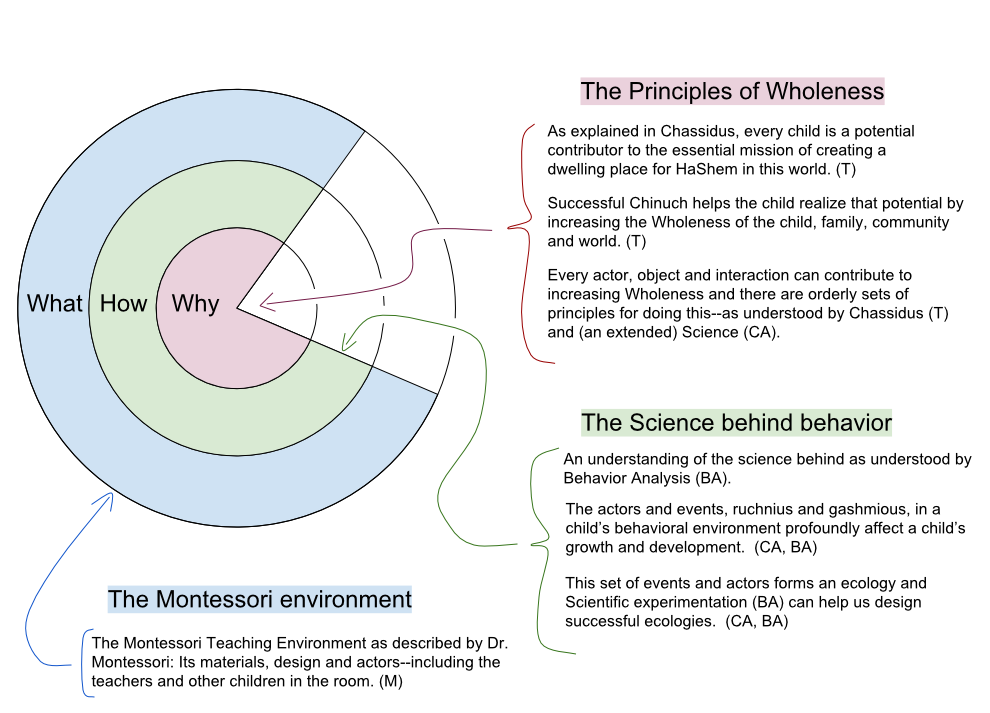
\includegraphics[scale=0.38]{graphics/onion-model-v2.png}
  \end{center}
\end{frame}

\begin{frame}
  \frametitle{Why: The Principles of Wholeness}
  \begin{itemizeLargerSpacing}
  \item As explained in Chassidus, every child is a potential
    contributor to the essential mission of creating a dwelling place
    for HaShem in this world. (T)
  \item Successful Chinuch helps the child realize that potential by
    increasing the wholeness of the child, family, community and
    world. (T)
  \item Every actor, object and interaction can contribute to
    increasing wholeness and there are orderly sets of principles for
    doing this--as understood by Chassidus (T) and (an extended)
    Science (CA).

  \end{itemizeLargerSpacing}

  \scriptsize{T = Torah; CA = Christopher Alexander; BA = Behavior
    Analysis; M = Montessori }
\end{frame}




\begin{frame}
  \frametitle{How: The Science behind the behavior}
  \begin{itemizeLargerSpacing}
  \item An understanding of the science behind behavior as understood
    by Behavior Analysis (BA).
  \item The actors and events--ruchnius and gashmious--in a child’s
    behavioral environment profoundly affect a child’s growth and
    development.  (CA, BA)
  \item This set of events and actors forms an ecology and scientific
    experimentation (BA) can help us design successful ecologies.
    (CA, BA)
  \end{itemizeLargerSpacing}
  \scriptsize{T = Torah; CA = Christopher Alexander; BA = Behavior
    Analysis; M = Montessori }

\end{frame}

\begin{frame}
  \frametitle{What: The Montessori environment}
  The Montessori Teaching Environment as described by Dr. Montessori.
  \begin{itemizeLargerSpacing}
  \item Its materials---the Montessori Works and their scripts
  \item Its design---how everything fits together in an integrated
    fashion
  \item Its (human) actors---the teachers and other children
  \end{itemizeLargerSpacing}
\end{frame}

\begin{frame}
  \frametitle{Chassidus: The Three Souls Model}
  \begin{center}
    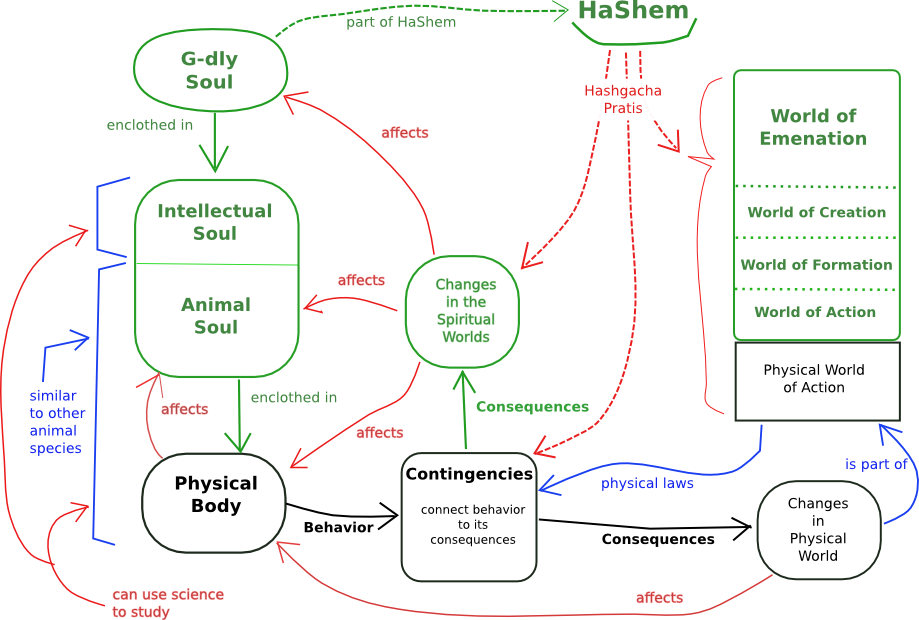
\includegraphics[scale=0.40]{graphics/chassidus-basic-model.png}
  \end{center}
\end{frame}
 \note{\scriptsize{
    \begin{itemize}
    \item Note 1: This is one of the most basic models in
      Chassidus. The G-dly soul is enclothed in the Intellectual Soul
      that is enclothed in Animal Soul that in turn is enclothed in
      the Body. Our job as Jews is for the G-dly soul to use the
      Intellectual Soul to train the Animal Soul to serve haShem---an
      animal training problem to train all 613 tricks with all their details.
    \item Note 2: Note that the G-dly soul needs the physical body to
      do physical mitzvahs in this world. Each physical action has
      many potential consequences in both the physical work and the
      spiritual worlds. The Torah is very much concerned with
      measurable behaviors---thought, speech and action. The
      contingencies are the ``rules'' that connect actions with
      consequences.
    \item Note 3: The interaction of HaShem with the spiritual and
      physical worlds is usually discussed in the context of ``filling
      all the worlds'' and ``surrounding all  the worlds.'' In this
      diagram it simply shown as ``hashgacha pratis.'' This will be
      identified with the ``Selectionist Model:'' The Darwin of
      Kedushah, so to speak.
    \end{itemize}} }



\begin{frame}
  \frametitle{Chassidus: Development and Change Models}
  \begin{center}
    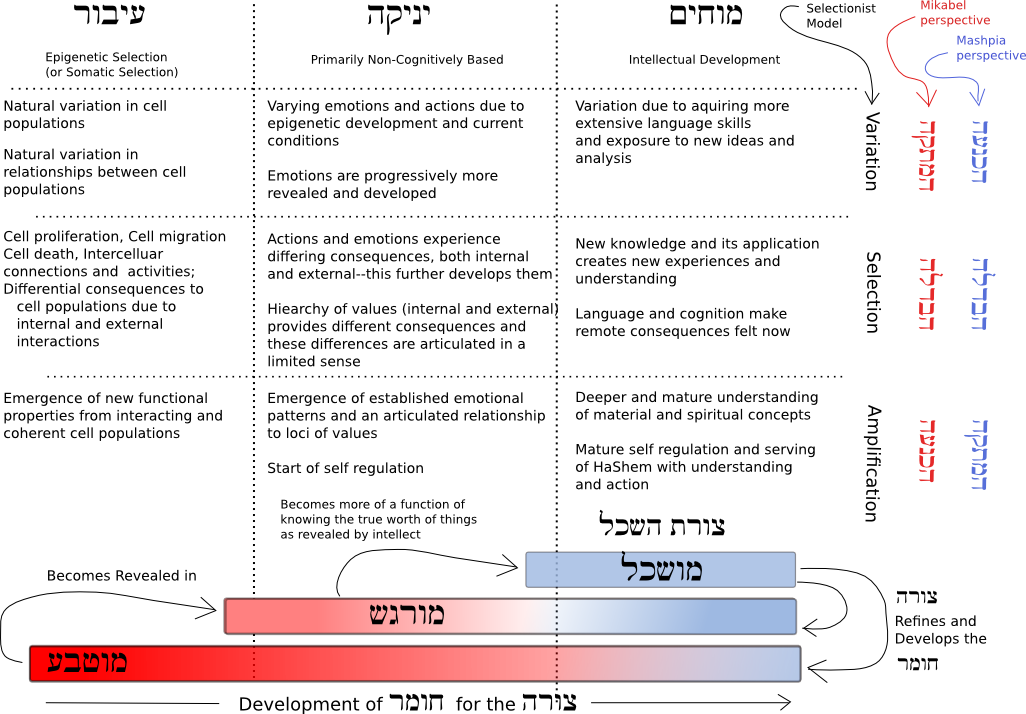
\includegraphics[scale=0.35]{graphics/development-change-chassidus-models.png}
  \end{center}
\end{frame}

 \note{\scriptsize{
    \begin{itemize}
    \item Note 1: In the book ``Absortent Mind'' Maria Montessori is very
      clear on what she is basing her models of learning and
      development. They are very closely related to evolutionary
      models of Darwin---as modified by De Vries. De Vries modifies
      Darwin's ideas to a non-gradualist model of evolution. Today the
      gradualist model of evolution is thoroughly
      unconvincing. Montessori largely applies this to an epigentic
      model of individual development. Her ``spiritual embryo'' is
      very much related to the selectionist model of epigensis. It
      roughly corresponds to the elements on this diagram.
    \item Note 2: The Selectionist model, as show in the diagram, corresponds to
      a well known model of the Baal Shem Tov: Subjugation, Separation,
      Sweetening. From the perspective of the Mashpia it goes in this order: (a)
      During the variation, the masphpiah doesn't mix in and the mikabel does
      ``what he wants;'' (b) During the selection phase the mashpia does create
      differential consequences; (c) during the amplification phase the mashpia
      drives it to fluency. This last part is ``sweet'' for the maspiah because
      the new fluent repertoire is acquired by the mikabal. It feels just the
      opposite to the mikabel. The first part (a) requires self control on the
      teachers part to not mix in---that is why it is the subjugation phase.

    \end{itemize}} }





\begin{frame}
  \frametitle{Two Examples from a Montessori Classroom}
  \begin{enumerate}
  \item A Child, lets call him Reuven, finished independent work and
    wants it corrected by teacher that is currently giving a lesson to
    three children on a rug. In the past Reuven has done many things
    to get a teachers attention. Many of them not according to the
    class rules. The class rule is that if a teacher is teaching a
    lesson a child has to stand quietly near the teacher with a hand
    on his shoulder to indicate that they want the teacher's
    attention.
  \item A Child in preschool, lets call him Simon, is using the pink
    tower work. This work has been just shown to him by a teacher. He
    is now using it for the first time by himself. Simon's hand
    coordination is OK but not as well developed as some other
    children in his class.

  \end{enumerate}

\end{frame}



\begin{frame}
  \frametitle{Selectionist Model}
  \begin{center}
    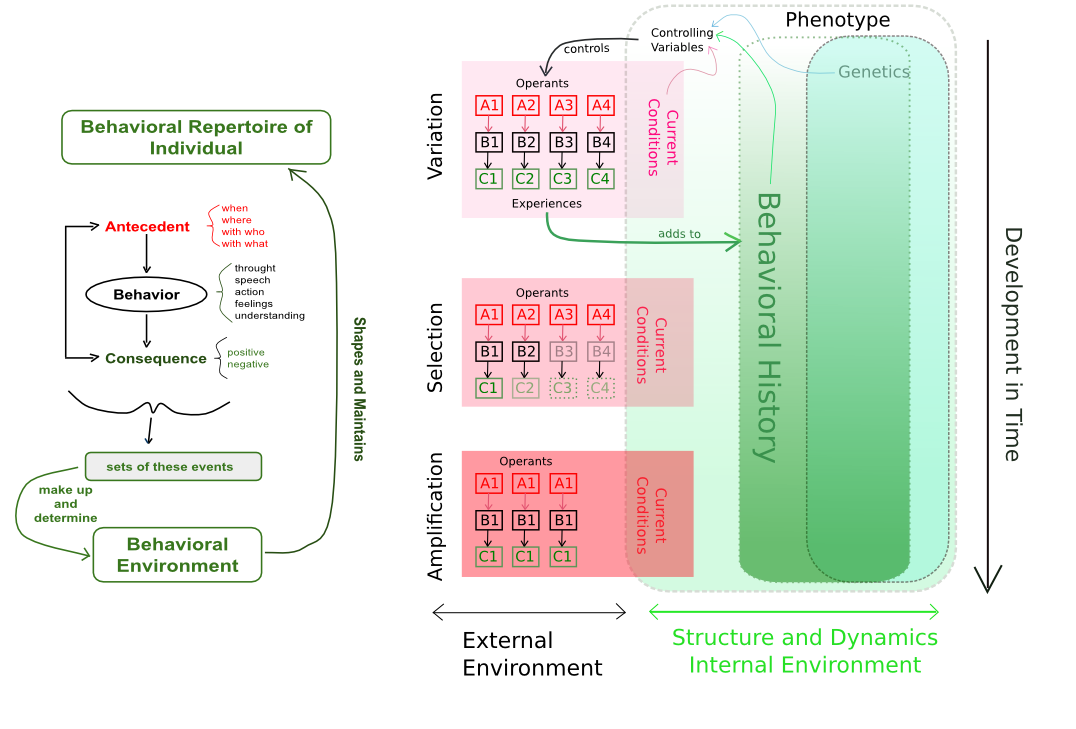
\includegraphics[scale=0.37]{graphics/Selectionist-Model.png}
  \end{center}
\end{frame}

 \note{\scriptsize{
    \begin{itemize}
    \item Note 1: Here we see many more details of the Selectionist
      model. Basically it helps develop the phenotype of the organism. In
      the diagram, the phenotype has as significant elements the
      genetics and behavioral history. Under the epigenetic model, the
      phenotype one cell population develops as a result of both its
      genetic controls and interaction with other cell populations
      under their genetic control, plus, the interactions with
      current environment.
    \item Note 2: In a certain very real sense the behavior history is part of
      the phenotype of the organism.
    \item Note 3: The diagram on the left shows a close up of the
      components of the operant, the classic three term contingency:
      In the presence of the antecedent a specific response class
      (behavior) is reinforced by a consequence.

    \end{itemize}} }

 \note{\scriptsize{
    \begin{itemize}
    \item Note 4: Here we see many more details of the Selectionist
      model. Basically it helps develop the phenotype of the organism. In
      the diagram, the phenotype has as significant elements the
      genetics and behavioral history. Under the epigenetic model, the
      phenotype one cell population develops as a result of both its
      genetic controls and interaction with other cell populations
      under their genetic control, plus, the interactions with
      current environment.
    \item Note 5: In a certain very real sense the behavior history is part of
      the phenotype of the organism.
    \item Note 6: The diagram on the left shows a close up of the
      components of the operant, the classic three term contingency:
      In the presence of the antecedent a specific response class
      (behavior) is reinforced by a consequence.

    \end{itemize}} }



\begin{frame}
  \frametitle{Selectionist Model: Variation}
  \begin{itemize}
    \small{
    \item Lets say that A1-B1-C1 corresponds to Rueven doing the right
      thing: quietly waiting next to the teacher with his hand on his
      shoulder while the teacher gives the lesson to the three other
      children
    \item A2-B2-C2, A3-B3-C3, A4-B4-C4 correspond to three ways of
      doing the wrong thing (e.g. saying over and over ``please
      correct this;'' or putting the paper in front of the teacher or
      bothering one of the children at the lesson)
    \item In this case, the antecedents are largely the same: A
      teacher is giving the lesson to three children and Rueven is
      nearby with his paper that needs correcting (so A1=A2=A3=A4).
    \item Lets assume the teacher does give Reuven the attention no
      matter what method he uses (So C1=C2=C3=C4.)  }
  \end{itemize}

\end{frame}

\begin{frame}
  \frametitle{Selectionist Model: Selection and Amplification}
  \begin{itemize}
    \small{
    \item Now the teacher changes the contigencies: He now longer pays
      any attention to Rueven unless he complies with the class rule.
    \item As can be seen on the diagram the other A2-B2-C2, etc are
      starting to fad out because their consequences are no longer
      occurring but Reuven still continues with B2, B3, B4 for a
      while.
    \item After some time exposed to this contingency, perhaps
      supplemented by some verbal praise that specifically appreciates
      the exact behaviors that Reuven is doing (``I really like how
      you waited so patiently even though I saw it was hard for
      you''), Reuven starts to use the ``right way'' of doing things
      to the exclusion of any other way of getting the teacher's
      attention. As we see in the lower part of the diagram. }
  \end{itemize}

\end{frame}
  



\begin{frame}
  \frametitle{Elements and Tactics---Why, How and What}
  \begin{center}
    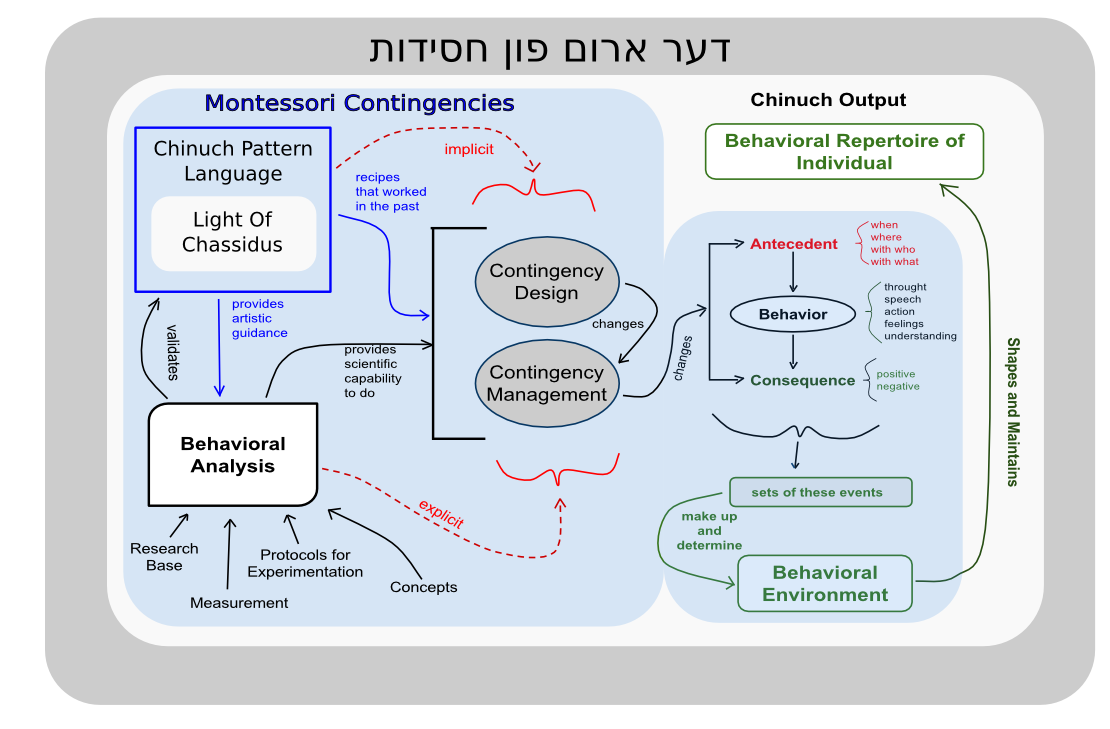
\includegraphics[scale=0.35]{graphics/Chinuch-ABA-elements.png}
  \end{center}
\end{frame}

 \note{\scriptsize{
    \begin{itemize}
    \item Note 1: This diagram now starts to put the selectionist model into a
      school based environment. The outer part of the onion is the
      actual implementation and it is in blue representing the fact
      that the Montessori contingencies largely are the ones used in
      the learning environment.
    \item Note 2: Chassidus appears in two places here: (a) as the
      inner light that guides the Chinuch Pattern Language; (b) the
      surrounding light that affects everything.
    \end{itemize}} }



\begin{frame}
  \frametitle{High Level Elements of Education}
  \begin{center}
    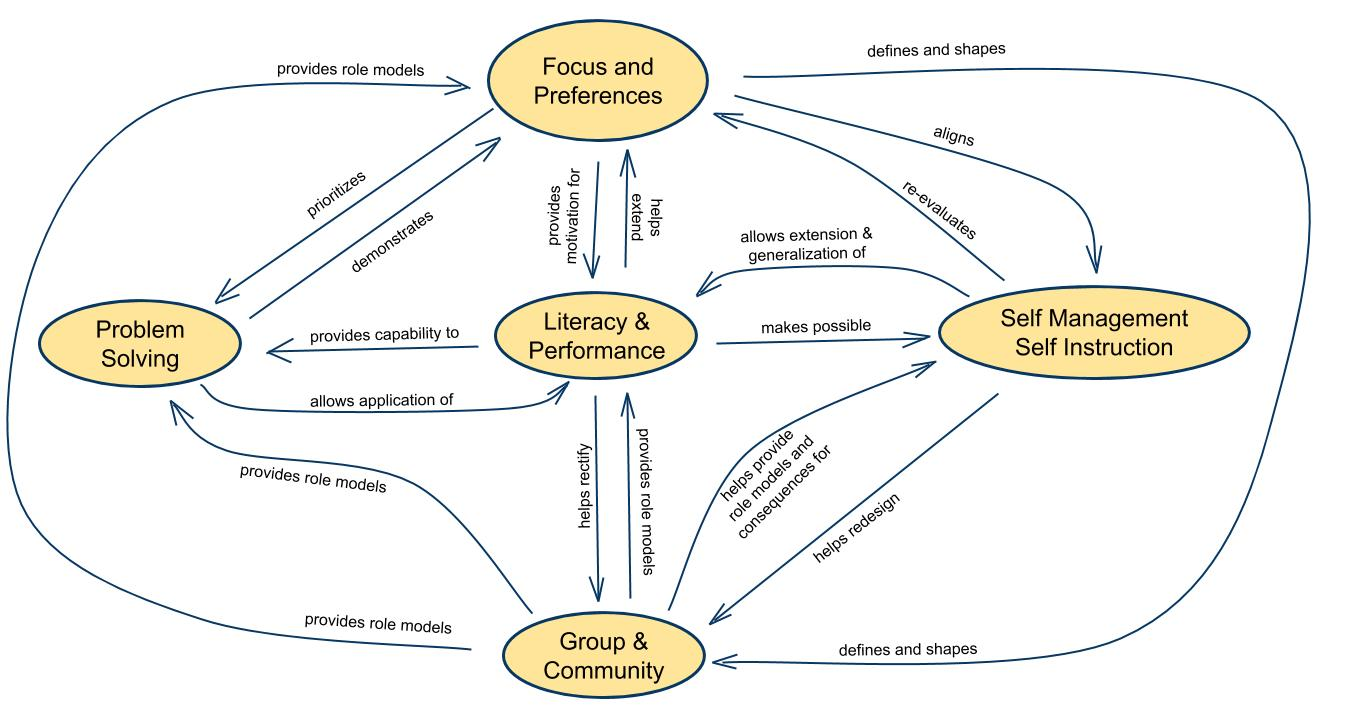
\includegraphics[scale=0.25]{graphics/Chinuch-ABA-elements-high-level.jpg}
  \end{center}
\end{frame}

 \note{\scriptsize{
    \begin{itemize}
    \item Note: Here we have the high level elements of the output
      of any successful educational system: secular or Jewish. Of
      course, in the case of Chinuch, each of the elements would have
      additional and important components. This is show in the next
      diagram.
    \end{itemize}} }



\begin{frame}
  \frametitle{Application to Chinuch---Literacy and Performance}
  \begin{center}
    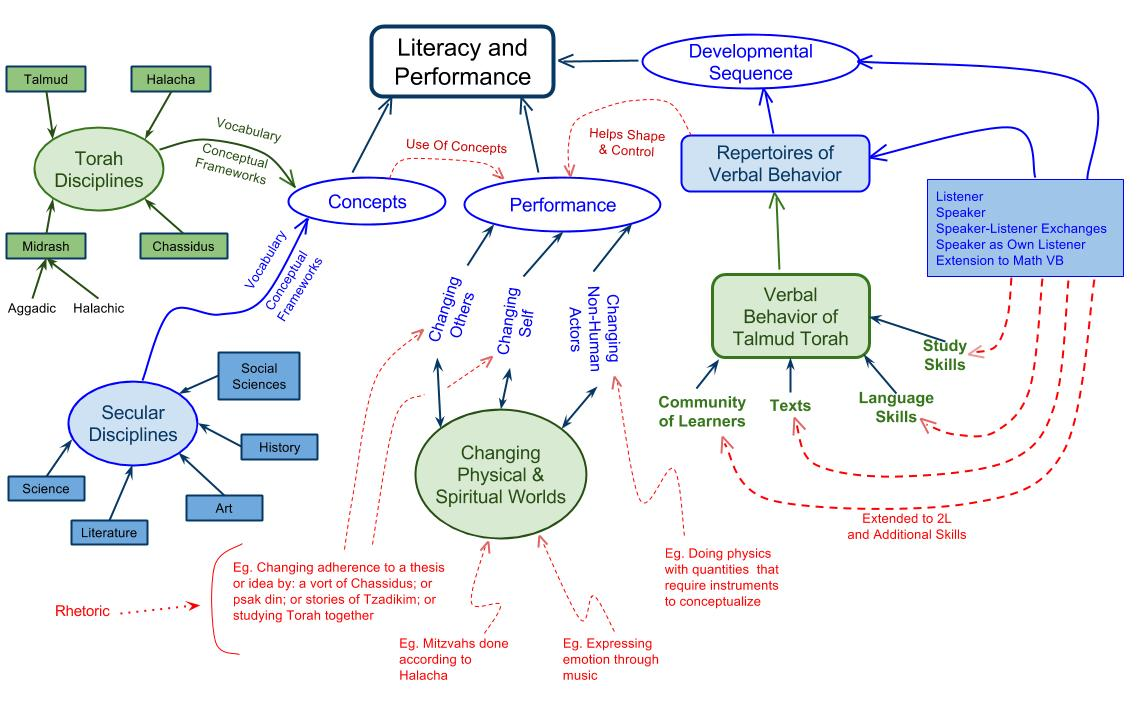
\includegraphics[scale=0.30]{graphics/Literacy-and-Performance.jpg}
  \end{center}
\end{frame}


\end{document}
% Local Variables:
% TeX-engine: xetex
% End:
